%!TEX root = ../../../FYP_Dissertation.tex

First of all, we are going to see how the JIT can make this object model
efficient and hoist away  all those costly lookups. In fact, the object model
described in the previous section might seem very slow as accessing variables
provided by a distant parent necessitates a big chain of lookups. In practice it
is not necessarily the case. Let's look at an example. Figure \ref{fig:MO-ex}
shows a model hierarchy that is transcribed in MAD by the lua code below from
lines 4 to 8. Since LuaJIT mainly compile loops, we are going to look at the IR
code (see Section \ref{Subsec:IR}) generated by LuaJIT for the loop lines 12 to 14
using the dump module (see Section \ref{Sec:Dump-mode}).

\begin{figure}[H]
    \centering
    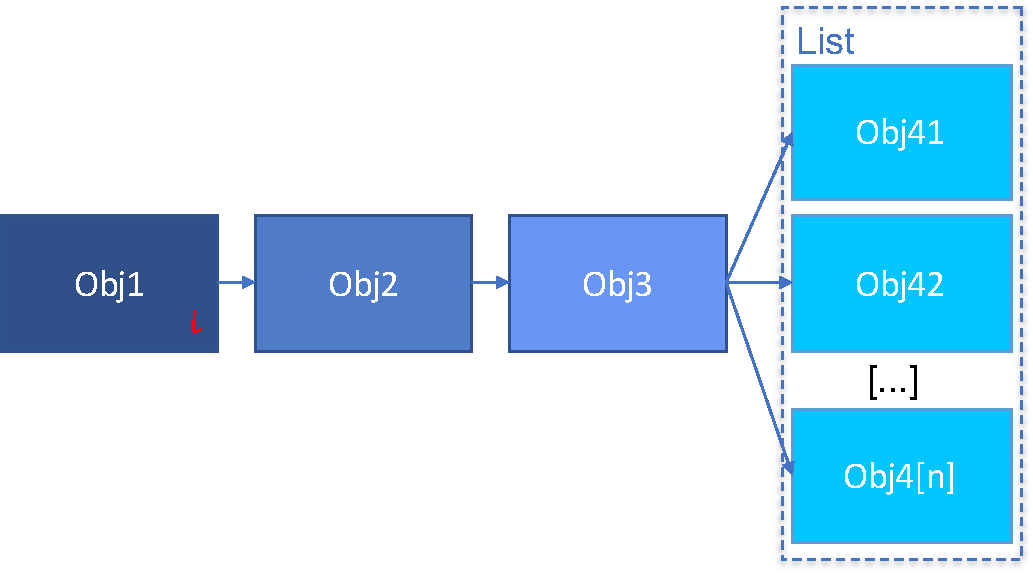
\includegraphics[width=0.8\textwidth]{./Images/MO-ex.pdf}
    \caption{Object inheritance of the example}
    \label{fig:MO-ex}
\end{figure}

\begin{lstlisting}[style=LuaStyle]
local object in MAD

-- object hierarchy
local obj1  = object "obj1"  { l = 42 }
local obj2  = obj1   "obj2"  { }
local obj3  = obj2   "obj3"  { }
local obj41 = obj3   "obj41" { }
local obj42 = obj3   "obj42" { }

-- loop
local sum = 0
for i=1,1e7 do
	sum = sum + obj41.l + obj42.l
end
\end{lstlisting}

\begin{figure}[H]
    \centering
    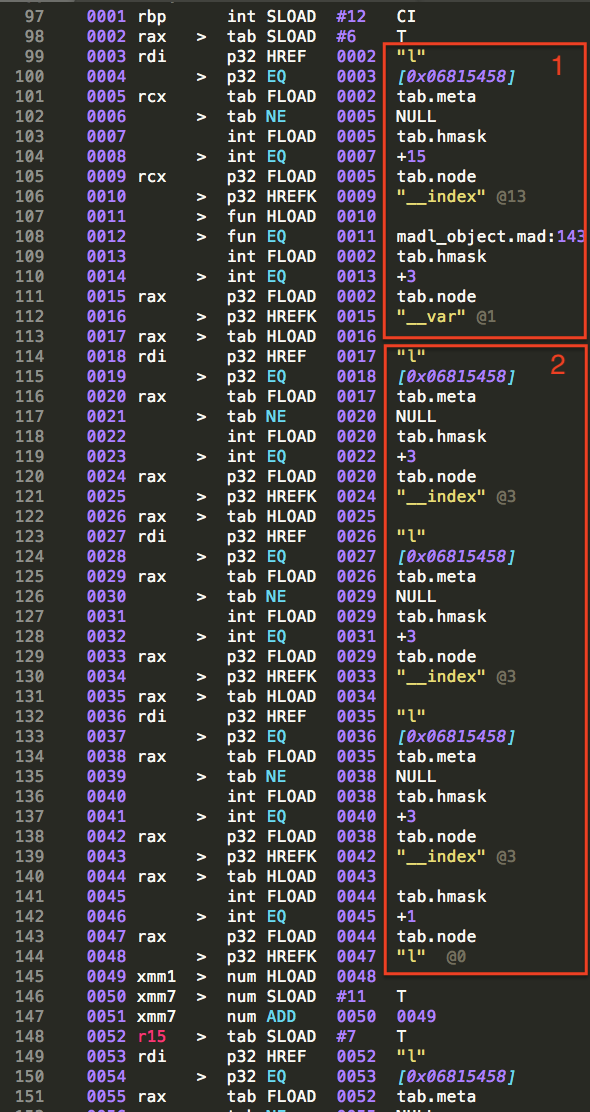
\includegraphics[height=13cm]{./Images/trace-1a}
    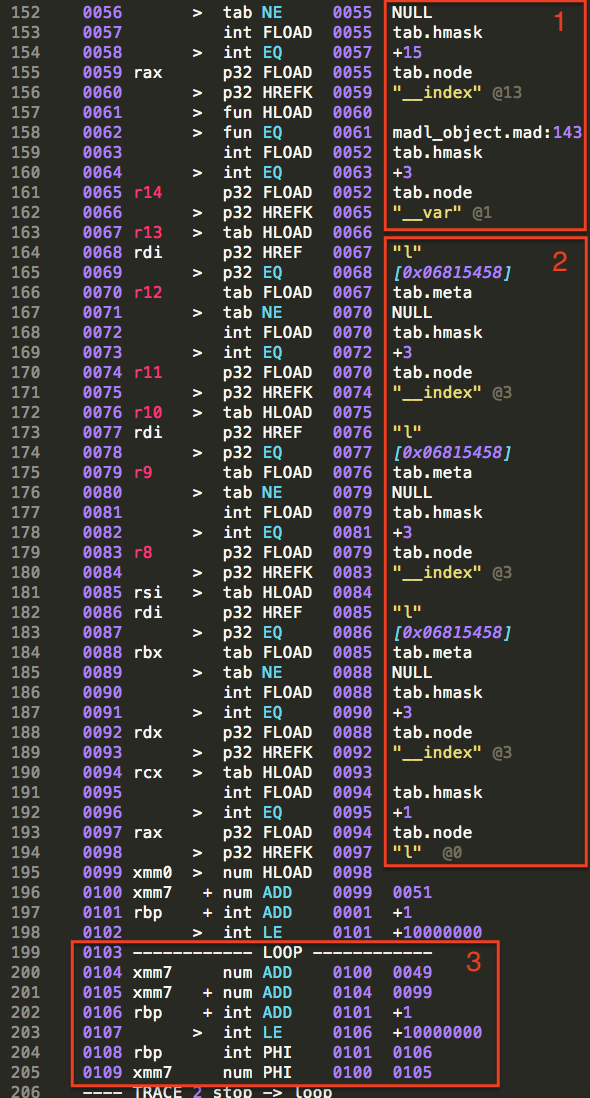
\includegraphics[height=13cm]{./Images/trace-1b}
    \caption{Screenshot of the example's loop trace}
    \label{fig:MO-ex-dump}
\end{figure}

Figure \ref{fig:MO-ex-dump} shows a screenshot of the dump trace. Without looking
at it too much in detail, we can see in the red squares labeled number one, the
access to the \emph{\_\_index} function that access the \emph{\_\_var} table to
query the "l" variable. Since this variable is not present in the first object
the hierarchy is unrolled three time (see the 3 "l" literals and the three
"\emph{\_\_index}" literals) in the red squares labeled with the number 2.
We have twice the same unrolling because the left screenshot shows the
unrolling for the first object (\emph{obj41}) and the right one shows the second
object (\emph{obj42}).

Now let's extract some general understanding from this example. Fist, the actual loop
is only the part in red labeled with the number three. We can see that it only
consists of the loop's counter and the additions. All other operations
from the model object has been successfully moved out of the loop making the loop
itself very small and efficient. This is the power of luaJIT. It can do that
using the loop optimization that consists of unrolling the loop once before the
actual loop itself executing all invariant operation and guards only once
(see \ref{Subsec:opt-loop} on loop optimization). Another thing to note here is
that the hierarchy chaining and the \emph{\_\_index} function is completely
inlined in the trace. This is always the case, there is never any explicit
control-flow possible in a trace with the exception of the actual LOOP currently
recorded, meaning that all functions and control-flow are inlined and specialized
to the runtime values.\\

Now let's look at another example based on the same hierarchy but slightly more
complex. Here the last level objects (\emph{obj4[n]}) are dynamic. Figure
\ref{fig:MO-ex-dump2} shows a screenshot of the dump trace for the second
example and we can clearly see that the hierarchy chaining is present both before
the loop (on the left) and inside the loop (on the right). This means that the
compiler hasn't been able to detect the invariance and produce a code similar to
the previous example, but it still manages to produce a single trace handling the
entire loop making it still performing better than with the VM interpreter.

\begin{lstlisting}[style=LuaStyle]
local object in MAD

-- object hierarchy
local obj1 = object "obj1" { l = 42 }
local obj2 = obj1   "obj2" { }
local obj3 = obj2   "obj3" { }

-- list of obj4[n]
local list = table.new(1e7, 0)
for i=1,1e7 do
	lists[i] = obj3 "obj4" {}
end

-- loop
local sum = 0
for i=1,1e7 do
	sum = sum + lists[i].l
end
\end{lstlisting}

\begin{figure}[H]
    \centering
    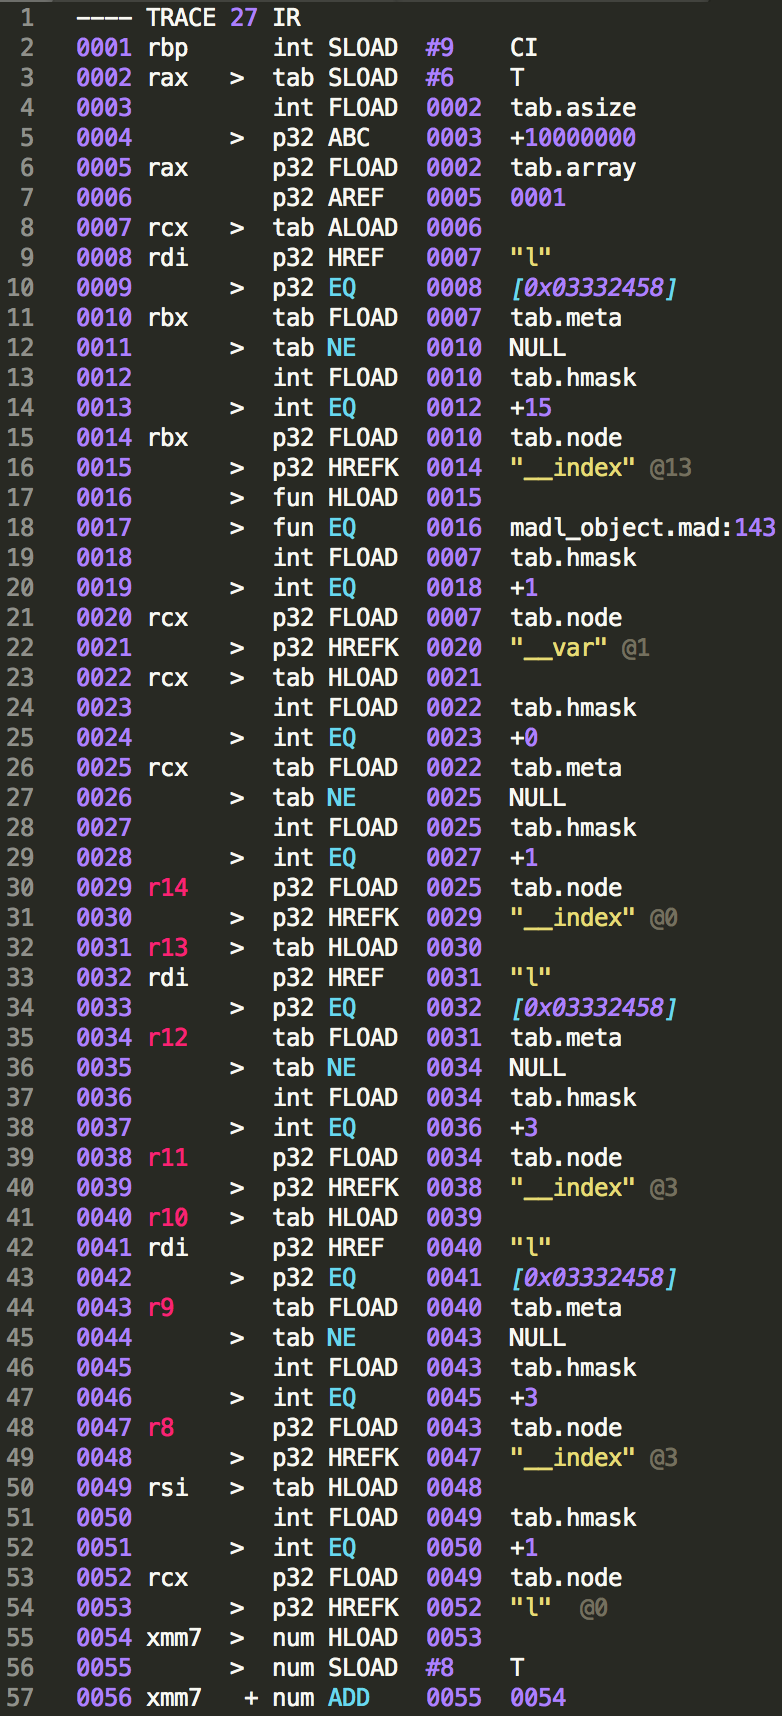
\includegraphics[height=13cm]{./Images/trace-2a}
    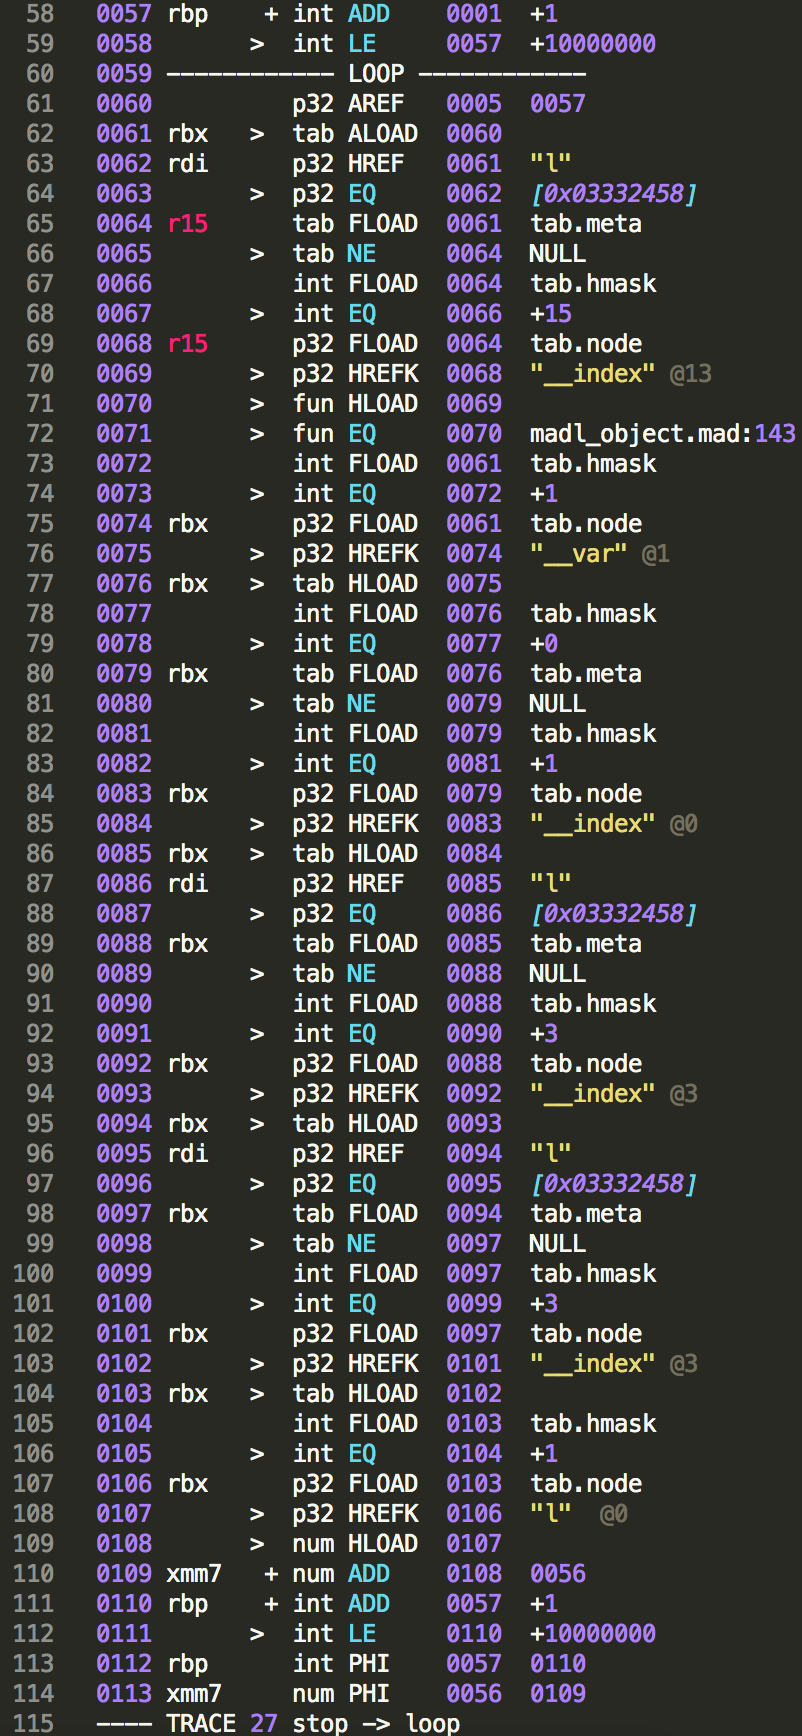
\includegraphics[height=13cm]{./Images/trace-2b}
    \caption{Screenshot of the second example's loop trace}
    \label{fig:MO-ex-dump2}
\end{figure}
